\subsubsection{Wstęp}
				\par Implementacje systemu komputerowego należy podzielić na środki programowe i sprzętowe. Do środków programowych zaliczamy oprogramowanie realizujące funkcjonalność opisanych w wcześniej składników systemu. Środkami sprzętowymi będą komputery oraz osprzęt sieciowy niezbędny do utworzenia sieci komputerowej.
				
			\subsubsection{Środki programowe}
				\par Korzystając z poprzednich informacji można ustalić podstawowy schemat komponentów programowych. System zarządzania oraz sklep internetowy muszą znajdować się na serwerze www. Oprogramowanie to jest odpowiedzialne za wygenerowanie dynamicznej strony internetowej na żądanie klienta lub pracownika sklepu. Następnym elementem będzie serwer wiadomości e-mail odpowiedzialny za komunikację elektroniczną. Kolejnym elementem systemu jest serwer centrali telefonicznej odpowiedzialny za połączenia przychodzące i wychodzące. Elementem wymaganym przez poprzednie składowe systemu jest serwer baz danych, na którym zapisywane będą dane pochodzące z poprzednich serwerów. Przedostatnim elementem jest serwer sieciowego systemu plików, na którym zapisywane będą dane pochodzące z serwera baz danych oraz wszystkie pozostałe pliki. Ostatnim elementem będą dwa serwery DNS, które są wymagane do samodzielnego przechowywania domeny.
				
				Lista serwerów potrzebnych do zrealizowania założeń obsługi klienta i funkcjonowania firmy: 
				\begin{itemize}
					\item Dwa serwery DNS
					\item Serwer wiadomości e-mail
					\item Serwer baz danych
					\item Centrala telefoniczna
					\item Serwer sieciowego systemu plików
					\item Serwer www
				\end{itemize}
			
				\par Na podstawie powyższej listy można przygotować podstawowy schemat systemu komputerowego. Należy rozszerzyć go o wcześniej nie wspomniane elementy jakimi są router i most sieciowy. Router'em nazywamy urządzenie komputerowe odpowiadające za trasowanie informacji na poziomie programowym do odpowiednich elementów systemu. Natomiast most sieciowy jest elementem spajającym wszystkie elementy sieci w spójną całość.
			
				\begin{figure}[H]
					\centering
					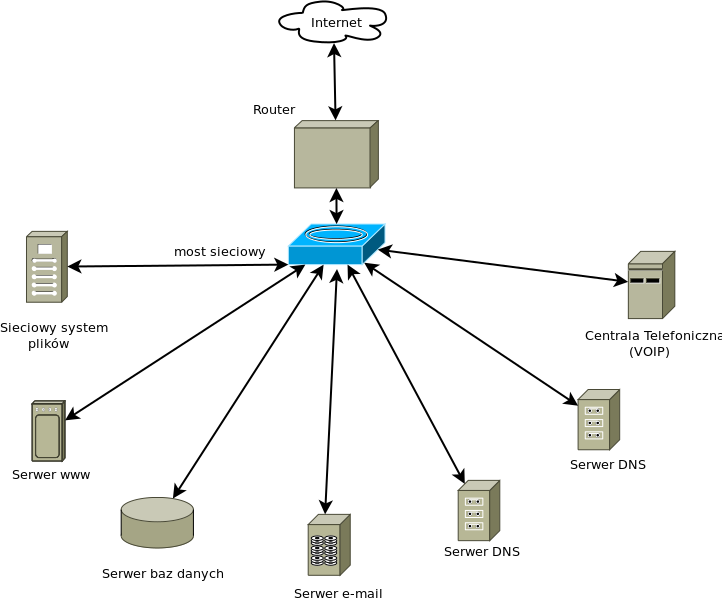
\includegraphics[scale=0.45]{Basic}
					\caption{Podstawowy schemat sieci}
					\label{basic_net}
				\end{figure}
				
				\par Serwery przedstawione na schemacie \ref{basic_net} mogą być komputerami fizycznymi lub komputerami wirtualnymi. Technologia wirtualizacji w systemach serwerowych pozwala utworzyć na komputerze fizycznym komputery wirtualne korzystające z jego zasobów. Innymi słowy na jednym fizycznym komputerze można uruchomić kilka komputerów wirtualnych. 
		
				\paragraph{Serwer wirtualny}
				\par Jako serwer wirtualny definiujemy proces umożliwiający uruchomienie komputera wirtualnie wraz z systemem operacyjnym pod kontrolą innego działającego już systemu operacyjnego. Serwer tego typu nazywany będzie serwerem VPS od angielskiego Virtual Private Server czyli wirtualnego serwera prywatnego.
		
			\subsubsection{Środki sprzętowe}	
				\par Do środków sprzętowych zaliczone zostaną komputery, router lub access point (AP), kasa fiskalna, oraz drukarka sieciowa. Poniższa lista w krótki sposób charakteryzuje wymienione sprzęty.
				
				\begin{description}
					\item[Serwery] - stanowią fundament firmy gdyż na nich znajdować się będzie sklep, centrala telefonii VOIP, serwis mailowy, infrastruktura sieci i bazy danych. Właśnie stąd sklep będzie hostowany na cały świat i to z serwerami będą łączyć się klienci.

					\item[Kasa fiskalna] - służy księgowaniu transakcji. Potrzebna będzie kasa walutowa pobierająca aktualne kursy walut, gdyż część transakcji będzie obejmowała klientów zagranicznych.

					\item[Przełącznik PoE] - urządzenie pozwalające na przyłączenie wielu urządzeń sieciowych do sieci komputerowej. Pozwoli to skonsolidować wszystkie elementy składowe sieci.

					\item[Macierz dyskowa] - komputer zawierający kilka dysków fizycznych przechowujących dane całej sieci. Dyski te połączone są w grupę "RAID", co gwarantuje bezpieczne przechowywanie dużych ilości danych. Takie rozwiązanie ma wymieniać dane pomiędzy serwerami, co zwiększa integralność sieci.

					\item[Drukarka sieciowa ze skanerem] - podstawowe wyposażenie biurowe; zestaw ten jest konieczny do drukowania, kserowania jak i skanowania dokumentów. 

					\item[Telefon voip] - telefon zostanie zastąpiony telefonią VOIP ze względu na wysokie stawki połączeń międzynarodowych przy standardowym połączeniu telefonicznym. Dzięki telefonii internetowej ze względu na używanie transferu opłaconego w abonamencie za usługi internetowe, będziemy mogli bez dodatkowych kosztów obsługiwać połączenia wychodzące jak i przychodzące.

					\item[Access Point] - pozwala na dostęp do sieci komputerowej za pomocą WiFi. Urządzenie to wykorzystywane będzie przez pracowników do podłączenia się do internetu jak i sieci lokalnej.
				\end{description}
				
				\par Jako serwer lub macierz dyskową należy rozumieć komputer świadczący w sieci komputerowej określone usługi na rzecz serwerów lub ludzi. Jako komputer należy rozumieć zespół połączonych ze sobą komponentów elektronicznych i elektromechanicznych jakimi są:
				
				\begin{description}
						\item{Procesor} - Elektroniczne urządzenie cyfrowe odpowiadające za pobieranie i przetwarzanie instrukcji. 
			
						\item{Płyta główna} - Element elektroniczny, na którym zamontowane są pozostałe podzespoły komputera. Umożliwia ona komunikację pomiędzy pozostałymi komponentami komputera.
			
						\item{Pamięć operacyjna} - Urządzenie elektroniczne umożliwiające przechowywanie wykonywanych programów, ich danych oraz wyników działania.
			
						\item[Dysk twardy] - Urządzenie elektroniczno-mechaniczne umożliwiające trwałe zapisanie wprowadzonych danych.
			
						\item[Karta sieciowa] - Komponent elektroniczny umożliwiający podłączenie komputera do sieci wraz z innymi komputerami i urządzeniami.
			
						\item[Karta graficzna] - Element elektroniczny umożliwiający wyświetlenie obrazu z komputera na odpowiednim wyświetlaczu.
			
						\item[Zasilacz] - Urządzenie elektromechaniczne dostarczające zasilanie do pozostałych podzespołów systemu komputerowego.
			
						\item[Obudowa] - Umożliwia umieszczenie i zamocowanie najważniejszych elementów komputera.
				\end{description}
				
				\subsubsection{Specyfikacja sieci}
					\par Wykorzystując wcześniej opracowane dane można przygotować specyfikację sieci prezentowaną przez schemat \ref{office}. Przedstawia ona środki sprzętowe niezbędne do zrealizowania wyznaczonych zadań.
			
					\begin{figure}[H]
						\centering
						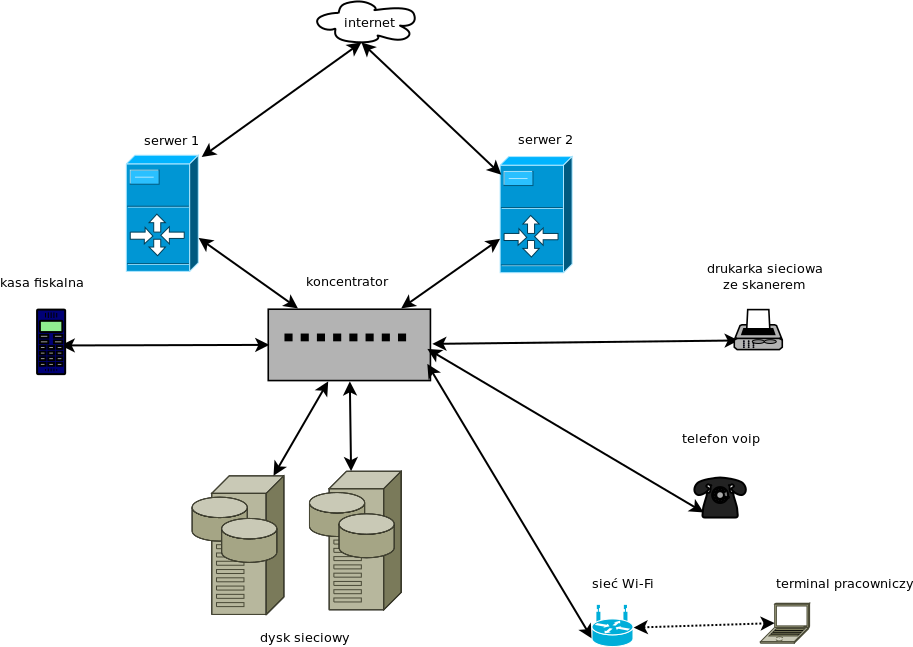
\includegraphics[scale=0.45]{Diagram1}
						\caption{Specyfikacja sieci biurowej}
						\label{office}
					\end{figure}
				
					\par Poniższy diagram przedstawia środki programowe niezbędne do realizacji założonych zadań umieszczone na dwóch serwerach, oraz współdzielony system plików na macierzy dyskowej. 
		
					\begin{figure}[H]
						\centering
						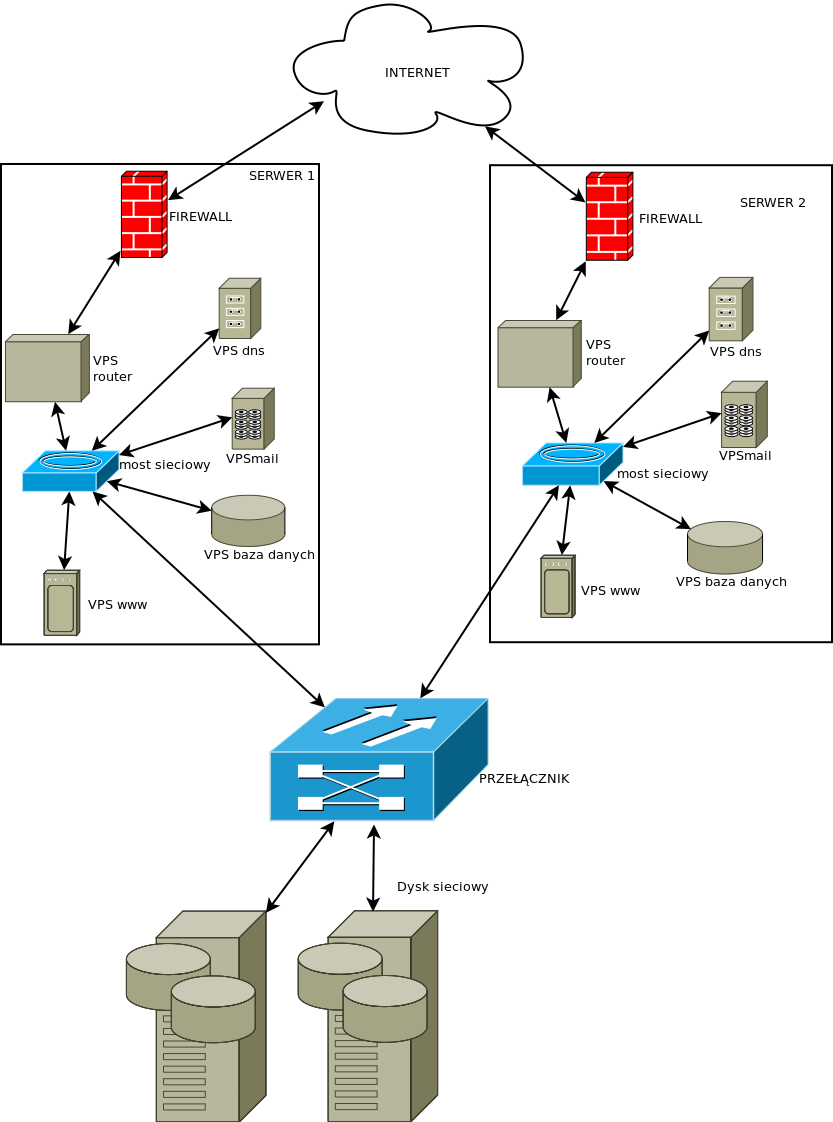
\includegraphics[scale=0.45]{Diagram2}
						\caption{Diagram środków programowych na serwerach}
						\label{net_real}
					\end{figure}
				
					\par Wykorzystana architektura systemu komputerowego nosi nazwę "failover cluster" wraz z technologią "load balancing". Jest to układ komputerów i oprogramowania, którego celem jest równoważenie obciążenia realizowanych zadań między zdublowane komponenty wykonujące te same funkcje. Oprócz tego umożliwia działanie systemu w przypadku awarii Serwera 1, lub Serwera 2, ze zmniejszoną wydajnością.
 
